%%
%%	Initial Management Report
%%	Created by Group02
%%
%%	10:27am 19/03/2013 
%%
%%	Use for SENG3011
%%

\documentclass[a4paper]{article}
\usepackage{a4wide}
\usepackage[normalem]{ulem} 
\usepackage{graphicx}
\usepackage{lscape}
\usepackage{float}

\begin{document}

%%%%%%%%%%%%%%%%%%%%%%%%%%%%%%%%%%%%%%%%%%%%%%%%%%%%%%%
%%TITLE PAGE
\thispagestyle{empty}
\begin {center}
\Large\textbf{SENG3011} 

\Large\textbf{Intial Management Report}

\bigskip\Large\textbf{Group Number: 02}

\end{center}

\vspace*{16.5cm}
\begin{tabular}{|l|l|}
  \hline
  Version         & 1.7\\\hline
  Print Date      & 19/03/2013 10:26\\\hline
  Release Date    & 27/03/2013\\\hline
  Release State   & Final \\\hline
  Approval State  & Pending \\\hline
  Approved by     & Group02 \\\hline
  Prepared by     & Group02 \\\hline
  Reviewed by     & Group02 \\\hline
  Confidentiality Category  & Confidential\\\hline
\end{tabular}
\pagebreak

%%%%%%%%%%%%%%%%%%%%%%%%%%%%%%%%%%%%%%%%%%%%%%%%%%%%%%%

%%%%%%%%%%%%%%%%%%%%%%%%%%%%%%%%%%%%%%%%%%%%%%%%%%%%%%%
%%REVISION CONTROL

\thispagestyle{plain}     % Turn on page numbering
\setcounter{page}{1}      % set page number counter
\renewcommand{\thepage}{\roman{page}}  % set page number to roman

\noindent{\Large\textbf{Document Revision Control}}\\[2ex]
\begin{tabular}{|l|l|l|l|}
  \hline
  Version & Date & Authors & Summary of Changes\\\hline\hline
	v1.0 & 20/03/2013 & Group02 & Added in Introduction           	\\\hline
	v1.1 & 24/03/2013 & Group02 & Added in Architectural Diagram 		\\\hline
	v1.2 & 25/03/2013 & Group02 & Added in Use Cases  		\\\hline
	v1.3 & 25/03/2013 & Group02 & Added in Sequence Diagrams		\\\hline
	v1.4 & 25/03/2013 & Group02 & Added in Model Architectural Diagram 		\\\hline
	v1.5 & 26/03/2013 & Group02 & Added in Project Plan		\\\hline
	v1.6 & 26/03/2013 & Group02 & Layout for Use Cases changed 		\\\hline
	v1.7 & 27/03/2013 & Group02 & Added in Justification of Chose Language and Envrionment 		\\\hline
\end{tabular}

\pagebreak

%%%%%%%%%%%%%%%%%%%%%%%%%%%%%%%%%%%%%%%%%%%%%%%%%%%%%%%

%%%%%%%%%%%%%%%%%%%%%%%%%%%%%%%%%%%%%%%%%%%%%%%%%%%%%%%
%%TABLE OF CONTENTS

\tableofcontents
\pagebreak
\listoffigures     %% delete if not required
\pagebreak         %% delete if there is no list of figures

%%%%%%%%%%%%%%%%%%%%%%%%%%%%%%%%%%%%%%%%%%%%%%%%%%%%%%%

%%%%%%%%%%%%%%%%%%%%%%%%%%%%%%%%%%%%%%%%%%%%%%%%%%%%%%%
%%MAIN

\setcounter{page}{1}     % Set page number counter
\renewcommand{\thepage}{\arabic{page}}  % print page number as arabic

\section {Introduction} 

This report is designed to discuss our initial prospects for the project and what we have in planned \\
for our final prototype. \\
\\ 
Within this report we will illustrate our Use Cases, Architecture and Sequence Diagrams,  \\
explain our chosen language and provide a project plan to which we hope to follow to   \\
complete our prototype.  \\
\\
We will be designing our report carefully following the Requirements List which has been \\
provided to us:  \\
\\
\indent\indent	1. Reading a correctly formatted Sirca orders file (1 day only) \\
\indent\indent 	2. Choosing an appropriate algorithmic trading strategy and setting its different \\
\indent\indent\indent	 		parameters \\
\indent\indent	3. Generating algorithmic orders for 1 particular day \\
\indent\indent	4. Evaluating algorithmic trades and providing feedback to the user \\
\indent\indent	5. Generating a strategy performance report \\ 
\indent\indent	6. GUI functions to control and use the Use Cases to load and execute orders \\ 
\indent\indent	7. GUI functions to visualise market data (spread, volume and depth) \\
\\
We will also aim to meet the Quality Requirements: \\
\\
\indent\indent	1. Speed of execution \\
\indent\indent 	2. Usability of the GUI \\
\indent\indent	3. Quality of the visualisation \\
\indent\indent	4. Quality of the strategic performance report \\	


\newpage	

\section {Use Cases}

From discussion between our members we were able to establish the following Use Cases: \\
\indent\indent	1. Placing a Bid Order	\\
\indent\indent	2. Placing an Ask Order 	\\	
\indent\indent	3. Amending a Bid Order 	\\
\indent\indent 	4. Amending an Ask Order \\	
\indent\indent	5. Deleting a Bid Order	\\
\indent\indent	6. Deleting an Ask Order 	\\ 
\\


\noindent{\bf Use Case 1}: Reading Correctly Formatted Sirca File \\
    \begin{tabular}{ | l | p{10cm} |}
    \hline
    	{\bf Actors} & User \\\hline
	{\bf Triggers} & The user starts the program. \\\hline
	{\bf Preconditions} & The user has a correctly formatted Sirca file. \\\hline
	{\bf Postconditions} & The system will be populated with orders \\\hline
	{\bf Normal Flow} & The system starts up, reads in the CSV file and\\
	& prepares the order book of trades.\\\hline
    \end{tabular} \\\\

\noindent {\bf Use Case 2}: Choosing an Algorithmic Trading Strategy \\ 
\begin{tabular}{ | l | p{10cm} |}\hline
	{\bf Actors} & User \\\hline
	{\bf Triggers} & User decides on a trade strategy to try.\\\hline
	{\bf Preconditions} & User has a decided quantity and strategy to trade with. \\\hline
	{\bf Postconditions} & System generates new orders based on specified quantity. \\\hline
	{\bf Normal Flow} & User indicates trading strategy, \\
	& system accepts trade strategy, generates the appropriate \\
	& bids and ask orders and sends it to the trade engine. \\\hline
\end{tabular} \\\\

\noindent {\bf Use Case 3}: Generating Trades for the Day \\ 
\begin{tabular}{ | l | p{10cm} |}\hline
	{\bf Actors} & User \\\hline
	{\bf Triggers} & User has chosen trading strategy and sent it to engine. \\\hline
	{\bf Preconditions} & Algorithmic trades are ready to process and a set of \\
	& orders have already been read in. \\\hline
	{\bf Postconditions} & All algorithmic trades are executed and ready for evaluation. \\\hline
	{\bf Normal Flow} & User tells system to continue with selected trades. \\
	& System executes the algorithmic trades and prepares for evaluation. \\\hline
\end{tabular} \\\\

\newpage
\noindent {\bf Use Case 4}: Evaluating Algorithmic Trades \\ 
\begin{tabular}{ | l | p{10cm} |}\hline
	{\bf Actors} & User \\\hline
	{\bf Triggers} & User wishes to determine the effectiveness of the strategy \\\hline
	{\bf Preconditions} & Algorithmic trades have been processed. \\\hline
	{\bf Postconditions} & The user is given feedback based on the algorithmic trades. \\\hline
	{\bf Normal Flow} & User asks for an evaluation, system finds the percentage gained or lost. \\\hline
\end{tabular} \\\\

\noindent {\bf Use Case 5}: Generating Strategy Performance Report \\ 
\begin{tabular}{ | l | p{10cm} |}\hline
	{\bf Actors} & User \\\hline
	{\bf Triggers} & User wants to see a performance report \\\hline
	{\bf Preconditions} & A strategy has been executed. \\\hline
	{\bf Postconditions} & A report will be generated for the user. \\\hline
	{\bf Normal Flow} & User asks system to generate strategy performance report. \\
	& System provides a performance report to the user.\\\hline
\end{tabular} \\\\

\begin {landscape}
\section {Architecture Diagram}
\begin{figure}[H]
  \centering
    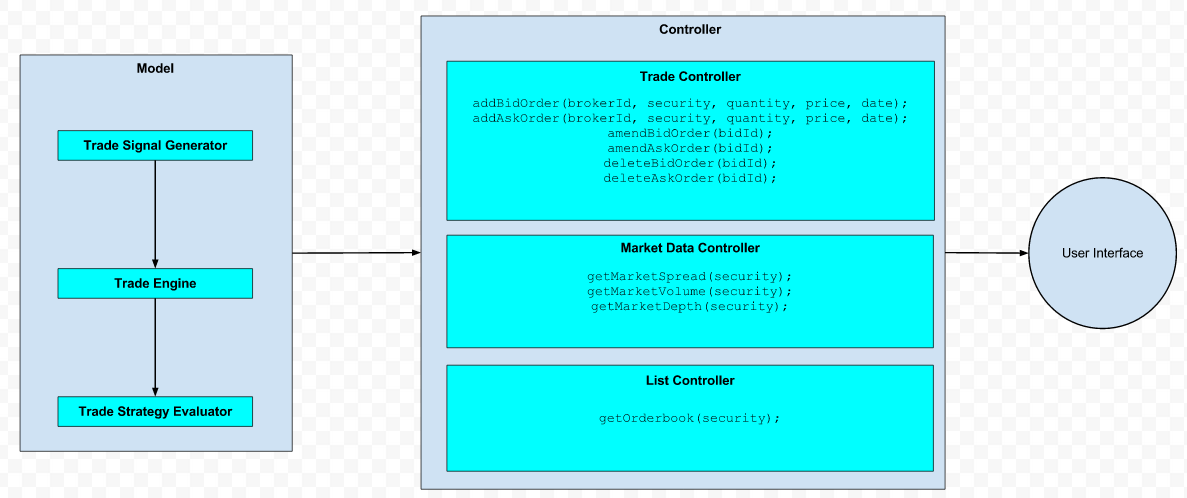
\includegraphics[width=1.6\textwidth]{images/ADiagram}
     \caption{Architectural Diagram.}
\end{figure}
\end {landscape}

\begin{landscape}
\begin{figure}
  
  \centering
    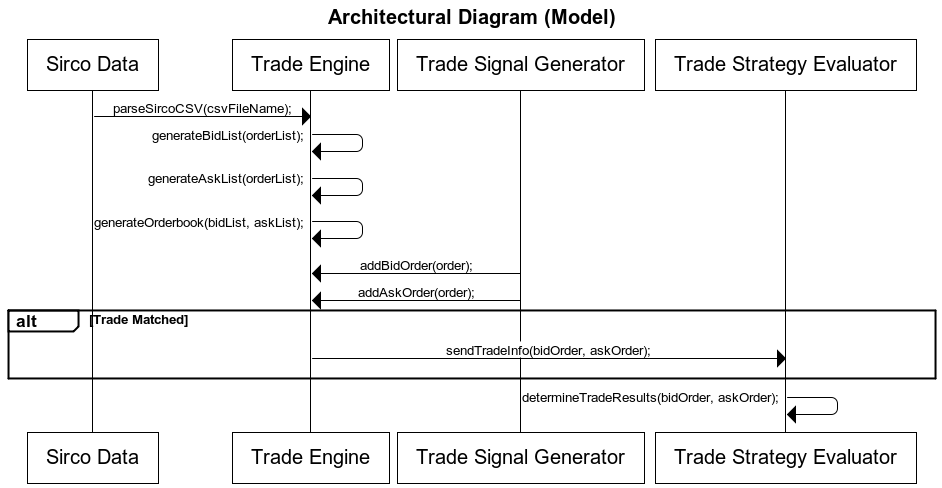
\includegraphics[width=1.6\textwidth]{images/aSequenceDiagram}
    \caption{Model Architectural Diagram.}
\end{figure}
\end {landscape}


\section {Sequence Diagram} 

The following are the Sequence Diagrams created created in parallel to the Use Cases \\
created by our team. \\

\begin{figure}[H] 
   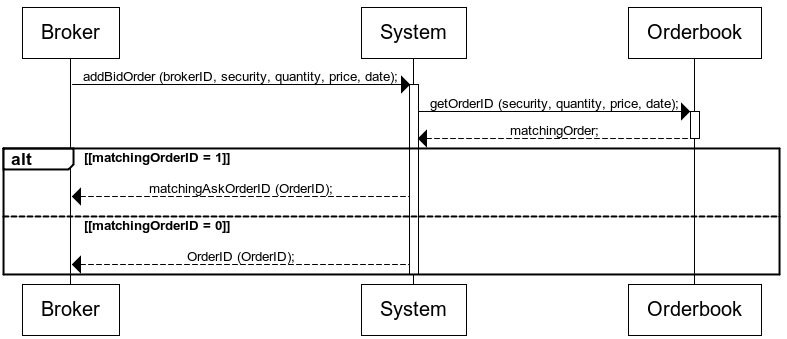
\includegraphics[width=1\textwidth]{images/addBidOrder}
   \caption{Use Case 1: addBidOrder}
\end{figure}

\begin{figure}[H]
   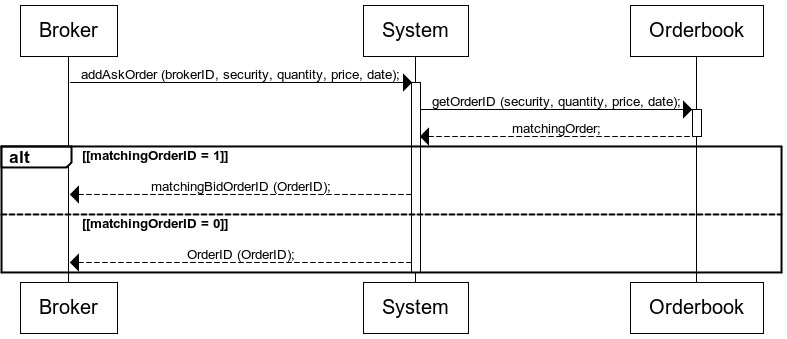
\includegraphics[width=1\textwidth]{images/addAskOrder}
   \caption{Use Case 2: addAskOrder}
\end{figure}

\begin{figure}[H]
   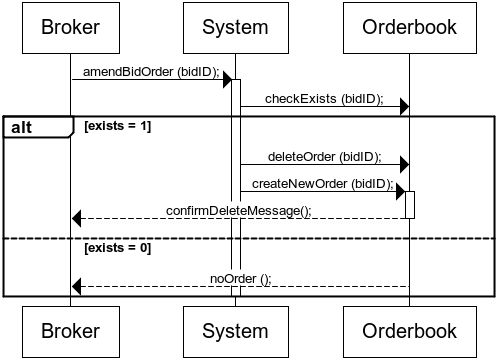
\includegraphics[width=1\textwidth]{images/amendBidOrder}
    \caption{Use Case 3: amendBidOrder}
\end{figure}

\begin{figure}[H]
   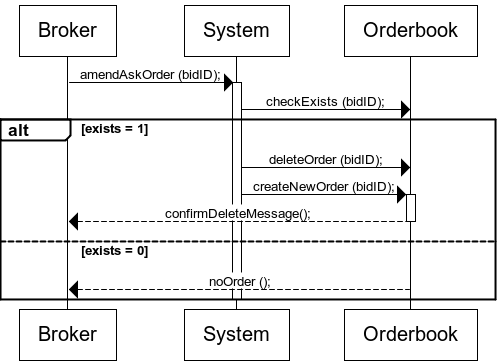
\includegraphics[width=1\textwidth]{images/amendAskOrder}
   \caption{Use Case 4: amendAskOrder}
\end{figure}

\begin{figure}[H]
   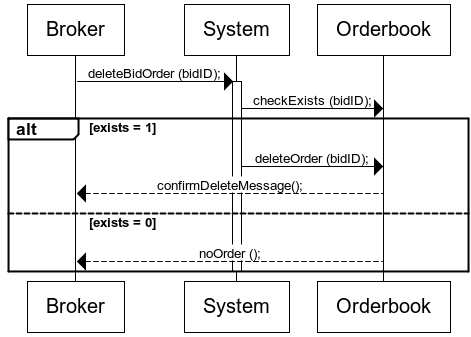
\includegraphics[width=1\textwidth]{images/deleteBidOrder}
   \caption{Use Case 5: deleteBidOrder}
\end{figure}

\begin{figure}[H]
   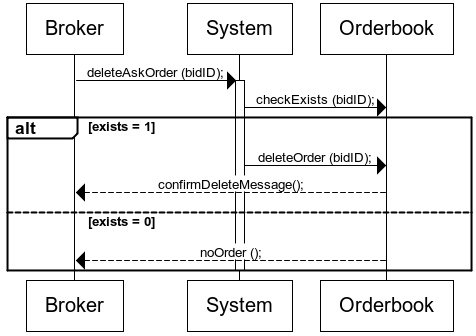
\includegraphics[width=1\textwidth]{images/deleteAskOrder}
   \caption{Use Case 6: deleteAskOrder}
\end{figure}

\section {Justification of chosen Language and Environment}

{\bf Development Environment}: \\
\indent Our language of choice is Java. Our decision to use Java is because of the extensive amount of \\ 
open source resources available for Java. Two resources we have already planned to use are \\
OpenCSV to read in the Sirco data and Swing to write our Graphical User Interface. Additionally, \\
we are more confident with Java in larger sized projects. Java also has an extensive amount  \\
of external resources and documentation. \\

\noindent {\bf Collaboration and version control}: \\
\indent We have decided to make use of Git and Github to maintain version control and collaborate 
our progress. We chose Git as it is a powerful version control tool and Github provides an  \\
informative interface to show past commits and if required, separate branches of our project. \\

\noindent {\bf Environment}: \\
\indent Everyone will be developing in Eclipse as it is quite a versatile and powerful open source IDE. \\
It is also extensively integrated with JUnit and will reduce some of the work required to set up \\
a testing environment for our system.

\section {Project Plan}

{\bf Communication}: 

\indent 1.  We will meet up every Tuesday, Wednesday and Friday for face to face updates and progress checking. \\
\indent 2. For most other times we will collaborate through our Facebook group page and \\
on Skype if conference calls are needed. \\
\indent 3. Google docs and other cloud software like LucidChart will be used for collaboration \\
 on report writing and diagrams. \\

\noindent {\bf Development Tools}:

\indent\indent 1. Eclipse is our IDE of choice. \\
\indent\indent 2. Our code will be in Java 6. \\
\indent\indent 3. Open source libraries like OpenCSV and Swing will be used. \\

\noindent {\bf Version Control}:

We are using Git to keep our projects up to date. \\

\noindent {\bf Roles}: \\
\indent\indent Sohaib Mushtaq - Developer, Tester \\
\indent\indent Shanku Roy - Developer, Quality Assurance \\
\indent\indent Michael Vuong - Developer, LaTeX/Report Generator \\
\indent\indent Albert Wang -  Developer, Team Lead \\

























\end {document}